\documentclass[letter, 11pt, twocolumn]{article}

\usepackage[utf8]{inputenc}
\usepackage[spanish]{babel}

\usepackage[left=0.75in,right=0.75in,top=0.75in,bottom=0.75in,columnsep=0.5in]{geometry}
\usepackage{graphicx}
\usepackage{float}
\usepackage{hyperref}

\usepackage{amsmath}
\numberwithin{equation}{section}

\usepackage{physics}

\usepackage{siunitx}
\DeclareSIUnit{\belmilliwatt}{Bm}
\DeclareSIUnit{\dBm}{\deci\belmilliwatt}
\DeclareSIUnit\lightyear{ly}
\newcommand*{\ra}[2][]{{% extra pair of braces for solution 1, doesn't hurt for solution 2
		%   \def\SIUnitSymbolDegree{\textsuperscript{h}}%     Solution 1
		%   \def\SIUnitSymbolArcminute{\textsuperscript{m}}%  Solution 1
		%   \def\SIUnitSymbolArcsecond{\textsuperscript{s}}%  Solution 1
		\ang[
		math-degree=\textsuperscript{h},             % Solution 2
		text-degree=\textsuperscript{h},             % Solution 2
		math-arcminute=\textsuperscript{m},          % Solution 2
		text-arcminute=\textsuperscript{m},          % Solution 2
		math-arcsecond=\textsuperscript{s},          % Solution 2
		text-arcsecond=\textsuperscript{s},          % Solution 2
		#1]{#2}%
}}
\usepackage{booktabs}
\usepackage{scrextend}
\def\tablename{Tabla}
\usepackage{stfloats}

% https://tex.stackexchange.com/questions/235783/listings-recognize-numbers-and-1e-3

\usepackage{xcolor}
\definecolor{maroon}{cmyk}{0, 0.87, 0.68, 0.32}
\definecolor{halfgray}{gray}{0.55}
\definecolor{ipython_frame}{RGB}{207, 207, 207}
\definecolor{ipython_bg}{RGB}{247, 247, 247}
\definecolor{ipython_red}{RGB}{186, 33, 33}
\definecolor{ipython_green}{RGB}{0, 128, 0}
\definecolor{ipython_cyan}{RGB}{64, 128, 128}
\definecolor{ipython_purple}{RGB}{170, 34, 255}

\usepackage{listings}
\renewcommand{\lstlistingname}{Código}
\lstset{
    breaklines=true,
    %
    extendedchars=true,
    literate=
    {á}{{\'a}}1 {é}{{\'e}}1 {í}{{\'i}}1 {ó}{{\'o}}1 {ú}{{\'u}}1
    {Á}{{\'A}}1 {É}{{\'E}}1 {Í}{{\'I}}1 {Ó}{{\'O}}1 {Ú}{{\'U}}1
    {à}{{\`a}}1 {è}{{\`e}}1 {ì}{{\`i}}1 {ò}{{\`o}}1 {ù}{{\`u}}1
    {À}{{\`A}}1 {È}{{\'E}}1 {Ì}{{\`I}}1 {Ò}{{\`O}}1 {Ù}{{\`U}}1
    {ä}{{\"a}}1 {ë}{{\"e}}1 {ï}{{\"i}}1 {ö}{{\"o}}1 {ü}{{\"u}}1
    {Ä}{{\"A}}1 {Ë}{{\"E}}1 {Ï}{{\"I}}1 {Ö}{{\"O}}1 {Ü}{{\"U}}1
    {â}{{\^a}}1 {ê}{{\^e}}1 {î}{{\^i}}1 {ô}{{\^o}}1 {û}{{\^u}}1
    {Â}{{\^A}}1 {Ê}{{\^E}}1 {Î}{{\^I}}1 {Ô}{{\^O}}1 {Û}{{\^U}}1
    {œ}{{\oe}}1 {Œ}{{\OE}}1 {æ}{{\ae}}1 {Æ}{{\AE}}1 {ß}{{\ss}}1
    {ç}{{\c c}}1 {Ç}{{\c C}}1 {ø}{{\o}}1 {å}{{\r a}}1 {Å}{{\r A}}1
    {€}{{\EUR}}1 {£}{{\pounds}}1
}

%%
%% Python definition (c) 1998 Michael Weber
%% Additional definitions (2013) Alexis Dimitriadis
%% modified by me (should not have empty lines)
%%
\lstdefinelanguage{iPython}{
    morekeywords={access,and,break,class,continue,def,del,elif,else,except,exec,finally,for,from,global,if,import,in,is,lambda,not,or,pass,print,raise,return,try,while},%
    %
    % Built-ins
    morekeywords=[2]{abs,all,any,basestring,bin,bool,bytearray,callable,chr,classmethod,cmp,compile,complex,delattr,dict,dir,divmod,enumerate,eval,execfile,file,filter,float,format,frozenset,getattr,globals,hasattr,hash,help,hex,id,input,int,isinstance,issubclass,iter,len,list,locals,long,map,max,memoryview,min,next,object,oct,open,ord,pow,property,range,raw_input,reduce,reload,repr,reversed,round,set,setattr,slice,sorted,staticmethod,str,sum,super,tuple,type,unichr,unicode,vars,xrange,zip,apply,buffer,coerce,intern},%
    %
    sensitive=true,%
    morecomment=[l]\#,%
    morestring=[b]',%
    morestring=[b]",%
    %
    morestring=[s]{'''}{'''},% used for documentation text (mulitiline strings)
    morestring=[s]{"""}{"""},% added by Philipp Matthias Hahn
    %
    morestring=[s]{r'}{'},% `raw' strings
    morestring=[s]{r"}{"},%
    morestring=[s]{r'''}{'''},%
    morestring=[s]{r"""}{"""},%
    morestring=[s]{u'}{'},% unicode strings
    morestring=[s]{u"}{"},%
    morestring=[s]{u'''}{'''},%
    morestring=[s]{u"""}{"""},%
    %
    % {replace}{replacement}{lenght of replace}
    % *{-}{-}{1} will not replace in comments and so on
    literate=
    {á}{{\'a}}1 {é}{{\'e}}1 {í}{{\'i}}1 {ó}{{\'o}}1 {ú}{{\'u}}1
    {Á}{{\'A}}1 {É}{{\'E}}1 {Í}{{\'I}}1 {Ó}{{\'O}}1 {Ú}{{\'U}}1
    {à}{{\`a}}1 {è}{{\`e}}1 {ì}{{\`i}}1 {ò}{{\`o}}1 {ù}{{\`u}}1
    {À}{{\`A}}1 {È}{{\'E}}1 {Ì}{{\`I}}1 {Ò}{{\`O}}1 {Ù}{{\`U}}1
    {ä}{{\"a}}1 {ë}{{\"e}}1 {ï}{{\"i}}1 {ö}{{\"o}}1 {ü}{{\"u}}1
    {Ä}{{\"A}}1 {Ë}{{\"E}}1 {Ï}{{\"I}}1 {Ö}{{\"O}}1 {Ü}{{\"U}}1
    {â}{{\^a}}1 {ê}{{\^e}}1 {î}{{\^i}}1 {ô}{{\^o}}1 {û}{{\^u}}1
    {Â}{{\^A}}1 {Ê}{{\^E}}1 {Î}{{\^I}}1 {Ô}{{\^O}}1 {Û}{{\^U}}1
    {œ}{{\oe}}1 {Œ}{{\OE}}1 {æ}{{\ae}}1 {Æ}{{\AE}}1 {ß}{{\ss}}1
    {ç}{{\c c}}1 {Ç}{{\c C}}1 {ø}{{\o}}1 {å}{{\r a}}1 {Å}{{\r A}}1
    {€}{{\EUR}}1 {£}{{\pounds}}1,
    %
    literate=
    *{+}{{{\color{ipython_purple}+}}}1
    {-}{{{\color{ipython_purple}-}}}1
    {*}{{{\color{ipython_purple}$^\ast$}}}1
    {/}{{{\color{ipython_purple}/}}}1
    {^}{{{\color{ipython_purple}\^{}}}}1
    {?}{{{\color{ipython_purple}?}}}1
    {!}{{{\color{ipython_purple}!}}}1
    {\%}{{{\color{ipython_purple}\%}}}1
    {<}{{{\color{ipython_purple}<}}}1
    {>}{{{\color{ipython_purple}>}}}1
    {|}{{{\color{ipython_purple}|}}}1
    {\&}{{{\color{ipython_purple}\&}}}1
    {~}{{{\color{ipython_purple}~}}}1
    %
    {==}{{{\color{ipython_purple}==}}}2
    {<=}{{{\color{ipython_purple}<=}}}2
    {>=}{{{\color{ipython_purple}>=}}}2
    %
    {+=}{{{+=}}}2
    {-=}{{{-=}}}2
    {*=}{{{$^\ast$=}}}2
    {/=}{{{/=}}}2,
    %
%   identifierstyle=\color{red}\ttfamily,
    commentstyle=\color{ipython_cyan}\ttfamily,
    stringstyle=\color{ipython_red}\ttfamily,
    keepspaces=true,
    showspaces=false,
    showstringspaces=false,
    %
    rulecolor=\color{ipython_frame},
    frame=single,
    frameround={t}{t}{t}{t},
    framexleftmargin=6mm,
    numbers=left,
    numberstyle=\tiny\color{halfgray},
    %
    %
    backgroundcolor=\color{ipython_bg},
    %   extendedchars=true,
    basicstyle=\scriptsize\ttfamily,
    keywordstyle=\color{ipython_green}\ttfamily,
    escapechar=\¢,escapebegin=\color{ipython_green},
}

\usepackage{rsc/long2}
\usepackage{titling}

\title{Informe Instrumentación Astronómica}
\author{Camilo Núñez Barra}

\begin{document}
\longtwocolumn[{
\begin{figure}[H]
	
\includegraphics[width=2in]{rsc/fcfm_das_eps}
\end{figure}
\begin{center}
	\textbf{\huge{INFORME\\CINEMÁTICA\\GALÁCTICA}}\\\,\\Tarea 2\\\,
\end{center}
\centering
\begin{tabular}{rl}
	Estudiante:&Camilo Núñez Barra\\
	RUT:&20.533.326-6\\
	Profesor:&Leonardo Bronfman\\
	Auxiliar:&Paulina Palma\\
	Curso:&AS3201 Astronomía Experimental\\
	Fecha:&\today\\
\end{tabular}
\vspace{1in}}]

\section{Introducción}

\subsection{Motivación}

La emisión de radiación electromagnética ha permitido descubrir la composición, cinemática y distribución del medio intergaláctico y estrellas.

La nubes frías de hidrógeno gaseoso no emiten luz visible sino ondas de radio. Estas nubes son importantes porque pueden indicar el lugar de nacimiento de estrellas.

La radioastronomía usa radiotelescopios que captan ondas de radio, de longitudes de aproximadamente \SI{1}{\centi\meter} a \SI{10}{\meter}. Favorablemente, estas ondas coinciden con una ventana en la atmósfera, permitiendo su detección. A pesar de esto, la atmósfera sigue teniendo opacidad, dando lugar a errores en la medición de las señales, al igual que el error sistemático provocado por el instrumento mismo y su receptor en la antena.

Este informe trata sobre, primero, ciertas calibraciones para el radiotelescopio que permiten mejorar la precisión de las mediciones y, en segundo lugar, sobre el estudio de la nebulosa de Orión.

\subsection{Estructura del Informe}

La sección \ref{sec:radiotelescopio} introduce el radiotelescopio y la sección \ref{sec:mini} el radiotelescopio utilizando en este informe. Las secciones \ref{sec:hotcoldtest} y \ref{sec:antennadipping} tratan sobre dos calibraciones para el telescopio, el Hot--Cold Test y Antenna Dipping, respectivamente, incluyendo un marco teórico, presentación de los datos medidos y cálculo de calibraciones, junto con la comparación con respecto a las provistas por el software del radiotelescopio. La sección \ref{sec:observaciones} introduce el objeto celeste observado, junto con los espectros, temperatura de la fuente y errores asociados. Finalmente, la sección \ref{sec:conclusiones} presenta las conclusiones del informe y la sección \ref{sec:anexo} es un anexo con los códigos utilizados para los cálculos y gráficos.

\subsection{El radiotelescopio}\label{sec:radiotelescopio}

Un radiotelescopio es una antena especializada en captar ondas de radio. Generalmente tiene una antena parabólica, con un reflector principal que redirige la radiación recibida del cielo, concentrándola en un reflector secundario pequeño y contrapuesto, que a su vez redirige la señal concentrándola en un pequeño receptor en la bocina de la antena.

La potencia espectral $w$ recibida por unidad de ancho de banda es,
\begin{equation}
w=\frac{1}{2}A_\textnormal{e}\iint_\Omega{B(\theta,\phi)P_n(\theta,\phi)\dd{\Omega}}\label{eq:w}
	,\end{equation}
donde $A_\textnormal{e}$ es la apertura efectiva de la antena, $B$ es el brillo del cielo, $P_n$ es el patrón de potencia normalizado de la antena que mide de la respuesta de sus lóbulos como función de los ángulos, y $\dd{\Omega}$ es el elemento infinitesimal de ángulo sólido del cielo. Además, el factor $1/2$ es debido a que la antena es responsable de una sola componente de polarización de la radiación.

\subsection{Radiotelescopio MINI}\label{sec:mini}

Los experimentos de este informe se realizan gracias a las mediciones hechas por el equipo docente mediante el radiotelescopio Southern Millimeter-Wave Telescope (ver figura \ref{fig:mini}), que ha permitido importantes investigaciones como un mapeo extenso y uniforme del carbolo interestelar de toda nuestra galaxias. Actualmente se usa para observaciones docentes, como la de este curso e informe.

Este telescopio se denomina MINI por su pequeño tamaño. Está en su propio domo en el Observatorio Astronómico Nacional, en la cima del cerro Calán. Su antena tiene un diámetro de \SI{1.2}{\meter}. Tiene instalado un amplificador HEMT (High Electro Mobility Transistor) en la primera etapa de recepción que proporciona una mejor relación señal a ruido. Tiene dos espectrómetros de banco de filtros con 256 canales cada uno, que captan ondas electromagnéticas con frecuencias d \SI{86}{\giga\hertz} a \SI{115}{\giga\hertz}, con resoluciones respectivas de \SI{0.1}{\mega\hertz} y \SI{1}{\mega\hertz}.

\begin{figure}[p]
	\centering
	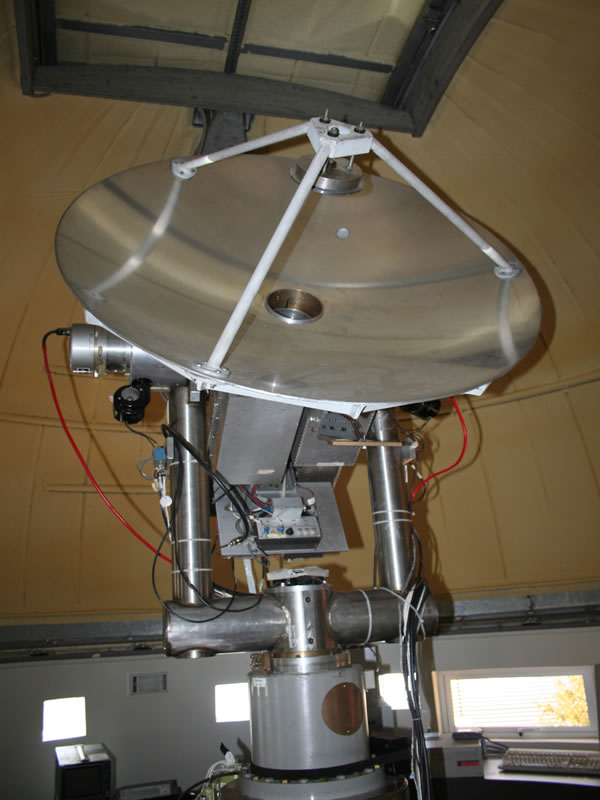
\includegraphics[width=3.25in]{mini.jpg}
	\caption{Radiotelescopio MINI (Imagen: DAS, FCFM)}
	\label{fig:mini}
\end{figure}

\begin{figure}[p]
	\centering
	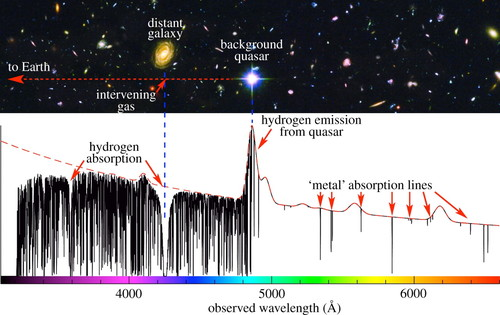
\includegraphics[width=3.25in]{spectrum.jpg}
	\caption{Espectro de absorción de un cuásar distante (Imagen: Joe Liske, ESO)}
	\label{fig:spectrum}
\end{figure}

\subsection{Espectros de absorción}

La potencia recibida (ecuación \ref{eq:w}) se puede recolectar a través de todos los canales del radiotelescopio, cada uno con una resolución determinada y un ancho de banda respectivo, permitiéndo graficarla en lo que se denomina espectro de absorción, como el que muestra la figura \ref{fig:spectrum}, que es para la luz visible pero sigue siendo ilustrativo para cualquiera. Las frecuencias o longitudes de ondas, adicionando su corrimiento debido al efecto Doppler, se pueden interpretar como velocidades radiales.

Una línea de absorción corresponde a un mínimo local preponderante en la curva del espectro y se producen porque los átomos en la línea de visión de la fuente se interponen en los fotones y absorben la energía para excitar sus electrones. Un ejemplo de absorción ocurre en las nubes de hidrógeno, que tienen temperaturas frías, y suelen indicar formación de estrellas.

Una línea de emisión corresponde a un máximo local preponderante en la curva del espectro y se produce por los fotones emitidos por las fuentes y los átomos que las componente. Un ejemplo de emisión ocurre en los cuásares y el hidrógeno que producen, estando a una muy alta temperatura.
\section{Curva de rotación}

\subsection{Marco teórico}

Sea $P$ un punto a través de la línea de visión a longitud $l$ y de distancia galactocéntrica $R=R_\odot\sin l$. Se supone $P$ bajo un movimiento puramente circular con velocidad $\vec{v}(R)$, denominada velocidad rotacional, cuya componente a lo largo de la línea de visión, es decir, su velocidad radial medible a través del efecto Doppler, es $\vec{v}_\parallel$, formando un ángulo $\alpha$ entre ambas, por lo tanto, contrarrestando la velocidad del Sol $\vec{v}_\odot$ relativa a la línea de visión,
\begin{equation}
v_\textnormal{LSR}(R)=v(R)\cos\alpha-v_\odot\sin l
.\label{eq:vll}\end{equation}
Sea $\beta$ el ángulo interior que forma el Sol, el punto $P$ y el centro galáctico. Se aprecia que $\beta=90+\alpha$, y, usando el teorema del seno,
\begin{equation}
\frac{\sin l}{R}\equiv\frac{\sin\beta}{R_\odot}=\frac{\cos\alpha}{R_\odot}
,\end{equation}
de modo que la ecuación \ref{eq:vll} se reescribe como,
\begin{equation}
v_\textnormal{LSR}(R)=v(R)\frac{R_\odot\sin l}{R}-v_\odot\sin l
,\label{eq:nomaestra}
\end{equation}
y, definiendo la velocidad angular mediante la siguiente relación,
\begin{equation}
v(R)=\omega(R)R
,\end{equation}
se obtiene la ecuación maestra de la cinemática de la Galaxia,
\begin{equation}
v_\textnormal{LSR}(R)=\left(\omega(R)-\omega(R_\odot)\right)R_\odot\sin l
.\label{eq:maestra}\end{equation}

Para una misma velocidad $v_\textnormal{LSR}(R)$, existe una doble ambigüedad en la distancia heliocéntrica $D$ del punto $P$ que le corresponde, pues, dentro del círculo solar, la línea de visión intersecta a la circunferencia de radio $R$ en un punto cercano y en otro lejano. Esto no ocurre fuera del círculo solar.

Es importante determinar la distancia $D$ para poder calcular la densidad numérica y densidad de masa gracias a la luminosidad, y, si no se determina, solo se puede calcular la densidad de columna.

Sea $D_\textnormal{N}$ la distancia cercana y $D_\textnormal{F}$ la distancia lejana. Geométricamente, se obtiene,
\begin{equation}
D_{\substack{F\\N}}=R_\odot\cos l\pm\sqrt{R^2-R_\odot^2\sin^2l}
\end{equation}

La velocidad máxima $v_\textnormal{LSR}^{\max}(R)$ que se puede medir en la línea de visión ocurre en el punto $P$ sobre esta que tiene la menor distancia galactocéntrica $R_{\min}=R_\odot\sin l$, suponiendo $\omega$ monotónicamente decreciente con respecto a $R$. Este punto se denomina punto subcentral. Su distancia heliocéntrica es $D_\textnormal{N}=D_\textnormal{F}=R_\odot\cos l=D_{\tan}$ y su velocidad tangencial o rotacional es, gracias a la ecuación \ref{eq:nomaestra}.
\begin{equation}
v_\textnormal{rot}(R_\odot\sin l)=v_\textnormal{LSR}(R_\odot\sin l)+v_\odot\sin l
,\label{eq:vrot}\end{equation}
y su velocidad angular es,
\begin{equation}
\omega(R_\odot\sin l)=\frac{v_\textnormal{LSR}}{R_\odot\sin l}+\omega(R_\odot)
.\label{eq:wrot}\end{equation}

Las velocidades rotacionales permitidas en la galaxia interna, en donde $R<R_\odot$ y luego $\omega(R)>\omega(R_\odot)$, para el cuarto cuadrante galáctico, en donde las longitudes está en el rango $\ang{270}<l<\ang{360}$, de modo que $\sin l<0$, cumplen, según la ecuación \ref{eq:maestra}, con $v_{\textnormal{rot}}<v(R)<0$.

\subsection{Detalle del algoritmo}

La curva de rotación se deriva de las velocidades terminales del espectro de CO para cada longitud galáctica $l$. El cuarto cuadrante galáctico tiene emisión con corrimiento al azul, por lo tanto, se escogen las velocidades terminales más negativas posibles para cada espectro y que cumplan cierta condición que se explica a continuación. El procedimiento corresponde al código X.

Se utiliza la técnica de \textit{sigma clipping} para obtener la base de ruido de los espectros con un número de 5 desviaciones estándar para el límite de recorte tanto superior como inferior, además de las iteraciones necesarias para que el algoritmo converja. Suponiendo que el promedio del ruido se anula, entonces la temperatura de ruido o valor RMS del ruido es igual a la desviación estándar del mismo.

La velocidad terminal se define para cada longitud $l$ y para cada latitud $b$ como aquella velocidad del primer punto del espectro de emisión cuya temperatura sea cinco veces mayor a la temperatura de ruido, considerando primero las velocidades del lado del corrimiento al azul del espectro, es decir, recorriendo el espectro desde la velocidad más negativa a la más positiva. Esta condición se muestra en la figura \ref{fig:vterminal}.

A continuación, se escoge para cada longitud $l$ el máximo maximorum entre las velocidades terminales de todas las latitudes $b$.

\begin{figure}[htbp]
	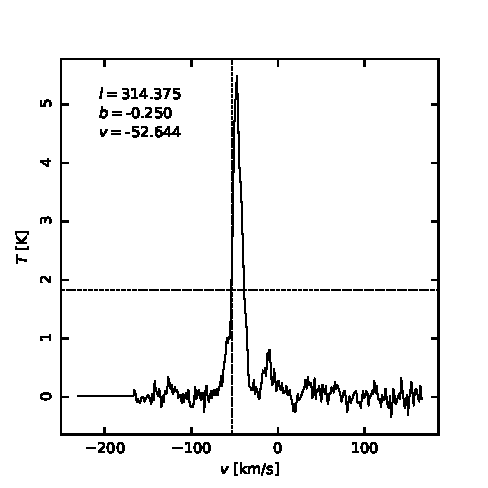
\includegraphics{rsc/vterminal.pdf}
	\caption{Un típico espectro de emisión, para las coordenadas $l=\ang{314.385}$ y $b=\ang{-0.250}$, con la condición para elegir la velocidad terminal. La línea discontinua horizontal representa un nivel de $5\sigma$ de ruido. La primera temperatura del lado del corrimiento al azul en superar esta condición ocurre a una velocidad $v_\textnormal{LSR}=\SI{-52.644}{\kilo\metre\per\second}$, que corresponde a la línea discontinua vertical.}
	\label{fig:vterminal}
\end{figure}

\subsection{Curva de rotación: $v_{\textnormal{rot}}$ vs. $R$ y \mbox{$\omega$ vs. $R$}}

Se usa la ecuación \ref{eq:vrot} y los máximos maximorum de velocidades terminales para graficar en la figura \ref{fig:vrot} las velocidades rotacionales para cada longitud.

Se utiliza la ecuación \ref{eq:wrot} junto con los máximos maximorum de velocidades terminales para graficar en la figura \ref{fig:vrot} las velocidades angulares para cada longitud.

\begin{figure}[htbp]
	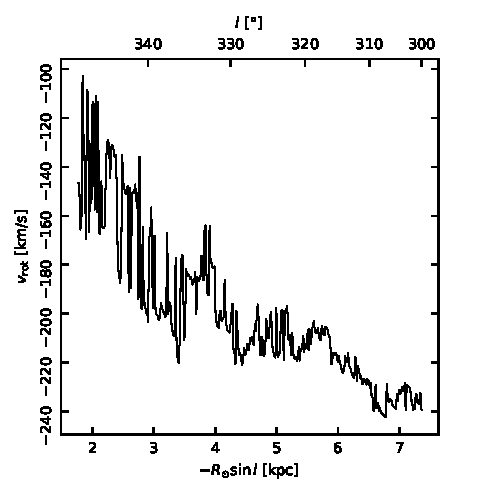
\includegraphics{rsc/vrot.pdf}
	\caption{Curva de rotación del cuarto cuadrante galáctico. Velocidad rotacional, correspondiente al máximo maximorum de velocidades terminales de las latitudes, en función de la distancia galactocéntrica (eje inferior) y la longitud (eje superior).}
	\label{fig:vrot}
\end{figure}

\begin{figure}[htbp]
	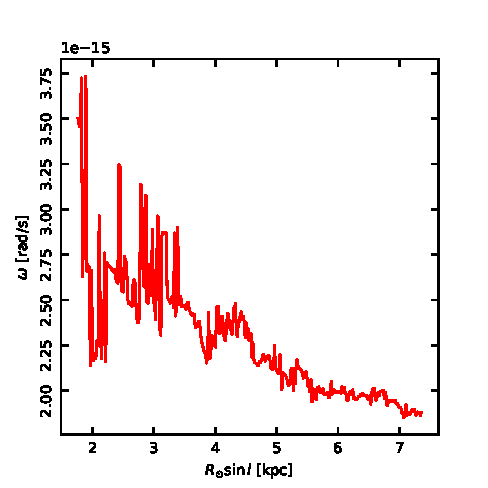
\includegraphics{rsc/w.pdf}
	\caption{Curva de rotación del cuarto cuadrante galáctico. Velocidad angular de cada máximo maximorum de velocidad terminal en función de la distancia galactocéntrica (eje inferior) y la longitud (eje superior).}
	\label{fig:w}
\end{figure}

\section{Corrugación del plano}

\subsection{Marco teórico}

El disco galáctico no es plano, sino que tiene una corrugación de aproximadamente \SI{150}{\parsec}, que es mucho menor comparado con los aproximadamente \SI{15}{\kilo\parsec} de radio. La corrugación de la altura $Z$ a través la distancia galactocéntrica $R$ se puede asimilar a un parche de un tambor de espesor minimal, puesto que la Galaxia tiene una estructura ondulatoria que depende en coordenadas cilíndricas de $\theta$ y $r$ y que funciona como una onda espiral de densidad, teniendo en $R$ modos normales de vibración, luego, se puede expresar analíticamente como una composición de funciones de Bessel, pero para este informe se hace un análisis más sencillo a partir de los datos medidos.

Gracias al algoritmo de la sección anterior, se toma como la posición de densidad máxima para cada longitud $l$ a la latitud $b$ donde se encuentra el máximo maximorum de velocidad terminal.

Se sabe también de la sección anterior que en este punto subcentral tangente al círculo, la distancia galactocéntrica es $D=R_\odot\sin l$ y la distancia heliocéntrica es $D=R_\odot\sin l$. Geométricamente, la altura para este punto respecto al ecuador galáctico es,
\begin{equation}
Z=R_\odot\sin l\tan b
,\label{eq:Z}\end{equation}
pudiendo aproximar $\tan b\approx b$ para pequeñas oscilaciones y mediciones.

\subsection{Detalle del algoritmo}

Se utiliza la latitud $b$ del máximo maximorum de velocidad para cada longitud $l$ del código \ref{cod:vrot} para calcular en el código \ref{cod:Z} la altura en cada longitud del disco según la ecuación \ref{eq:Z}. 

\subsection{Corrugación del plano: $Z$ vs. $R$}

La figura \ref{fig:Z} muestra la corrugación del disco galáctico en función del radio galactocéntrico.

\begin{figure}[htbp]
	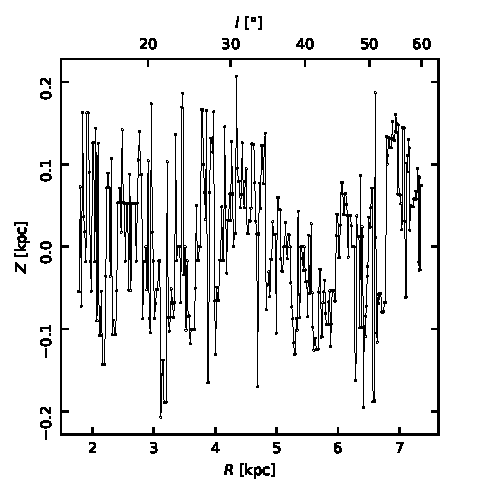
\includegraphics{rsc/Z.pdf}
	\caption{Corrugación del plano. Altura $Z$ de cada punto subcentral con respecto a la distancia galactocéntrica (eje inferior) y la longitud correspondiente (eje superior).}
	\label{fig:Z}
\end{figure}

\section{Ajuste de modelo de masa}

\subsection{Marco teórico}

Se quiere encontrar una fórmula analítica para la curva de rotación basándose en un modelo físico que considere la distribución de masa de la galaxia.

Se iguala para cierta partícula de masa $m$ en rotación pura la fuerza de gravedad con la fuerza centrípeta,
\begin{equation}
G\frac{M(R)m}{R^2}=m\frac{v_\textnormal{rot}^2(R)}{R}
,\end{equation}
donde $G$ es la constante de gravitación universal y $M$ es la masa de la galaxia dentro de un radio $R$ determinado por la distancia galactocéntrica de la partícula. Luego, la velocidad de rotación de la curva de rotación de la figura \ref{eq:vrot} se puede modelar por,
\begin{equation}
v_\textnormal{rot}(R)=\sqrt{G\frac{M(R)}{R}}
.\label{eq:vmass}\end{equation}

Se estudian cinco modelos de distribución de masa para la galaxia, listados a continuación.
\begin{itemize}
\item Masa puntual en el centro de la galaxia. $M(R)=M_0$. $M_0$ es el parámetro libre de la masa puntual.

\item Disco uniforme. $M(R)=\pi R^2s_0$. $s_0$ es el parámetro libre de densidad superficial uniforme de masa.

\item Esfera uniforme. $M(R)=\frac{4}{3}\pi R^3\rho_0$. $\rho_0$ es el parámetro libre de densidad uniforme volumétrica de masa.

\item Disco uniforme con una masa puntual en el centro. $M(R)=\pi R^2s_0+M_0$. Dos parámetros libres, $s_0$ y $M_0$.

\item Esfera uniforme con una masa puntual en el centro. $M(R)=\frac{4}{3}\pi R^3\rho_0+M_0$. Dos parámetros libres, $rho_0$ y $M_0$.
\end{itemize}

\subsection{Detalla del algoritmo}

El código X muestra el sigueinte procedimiento. Se evalúan los cinco modelos de distribución de masa en la ecuación \ref{eq:vmass} y se realiza un ajuste no lineal de mínimos cuadrados según el algoritmo de Levenberg-Marquardt para cada modelo, asumiendo una desviación estándar de la unidad para las velocidades de rotación. Además, se calcula el error RMS de cada modelo con respecto a las velocidades de rotación medidas para determinar el mejor ajuste.

\subsection{Ajuste de los modelos de la curva de rotación}

La tabla \ref{tab:massmodel} muestra el resultado del ajuste de mínimos cuadrados con los parámetros óptimos para cada modelo de distribución de masa de la Galaxia y el error RMS con respecto a la velocidad rotacional medida.

La figura \ref{fig:massmodel} muestra el gráfico de los ajustes de los cinco modelos de distribución de masa de la Galaxia.

\begin{table*}[htpb]
	\centering
	\begin{tabular}{lcccc}
		\toprule
		{Modelo} &
		{$M_0$} &
		{$s_0$} &
		{$\rho_0$} &
		{RMS} \\
		{} &
		{$\textnormal{M}_\odot$} &
		{$\textnormal{M}_\odot\,\textnormal{kpc}^{-2}$} &
		{$\textnormal{M}_\odot\,\textnormal{kpc}^{-3}$} &
		{\si{\kilo\meter\per\second}} \\
		\midrule
		Punto & $3.655\times10^{10}\pm1.321\times10^{9}$ & --- & --- & $68.738$ \\
		Disco & --- & $6.419\times10^{8}\pm5.501\times10^{6}$ & --- & $17.248$ \\
		Esfera & --- & --- & $8.569\times10^{7}\pm1.883\times10^6$ & $43.337$ \\
		Disco + Punto & $3.928\times10^{9}\pm3.422\times10^{8}$ & $5.814\times10^{8}\pm6.851\times10^{6}$ & --- & $14.749$ \\
		Esfera + Punto & $1.259\times10^{10}\pm4.343\times10^{8}$ & --- & $6.127\times10^{7}\pm1.112\times10^{6}$ & $21.326$ \\
		\bottomrule
	\end{tabular}
	\caption{Parámetros y error obtenido del ajuste no lineal de míminos cuadrados para los modelos de distribución de masa de la Galaxia con respecto a la velocidad rotacional medida.}\label{tab:massmodel}
\end{table*}

\begin{figure}[htbp]
	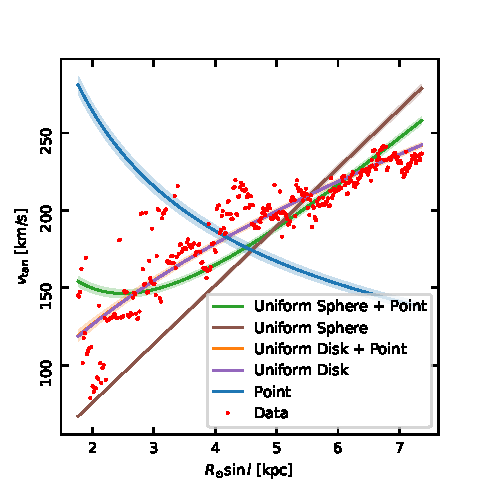
\includegraphics{rsc/massmodels.pdf}
	\caption{Ajuste de los modelos de distribución de masa de la Galaxia con respecto a la curva de rotación medida. Línea negra es datos medidos. Línea naranja es modelo de masa puntual central. Línea verde es modelo de disco uniforme. Línea naranja es modelo de esfera uniforme. Línea azul es modelo de disco uniforme con masa puntual central. Línea morada es modelo de esfera uniforme con masa puntual central. Las cinco líneas de ajustes tienen un área respectiva que representa el error de los parámetros óptimos.}
	\label{fig:massmodel}
\end{figure}
\section{Análisis y conclusiones}

La figura \ref{fig:vrot} muestra que la velocidad rotacional de los puntos subcentrales es globalmente creciente con respecto al radio galactocéntrico. Sin embargo, localmente se aprecian alternadas fluctuaciones de aproximadamente \SI{50}{\kilo\metre\per\second} hasta alcanzar un radio de \SI{4}{\kilo\parsec}, y esto se explica porque la línea de visión cercana centro de la Galaxia atraviesa más nubes de gas y en el centro se producen colapsos y expansiones, aumentando la distribución de velocidades.

A partir de aproximadamente \SI{4}{\kilo\parsec} de radio, la magnitud de las fluctuaciones de la velocidad rotacional disminuye, a la vez que se aumenta la velocidad.

La velocidad rotacional pareciera ser aproximadamente constante para longitudes menores a \ang{310}.

La figura \ref{fig:w} muestra que la curva de rotación concuerda con que la galaxia presenta una rotación diferencial, puesto que la velocidad angular de los puntos subcentrales disminuye con la distancia galactocéntrica. Se aprecia también el mismo fenómeno anterior de fluctuaciones para radios menores.

La mayor velocidad angular para radios menores indica que una rotación completa de esa zona de la galaxia demora 66370000 años, mientras que para radios mayores la rotación completa demora 199100000 años. Además, la tendencia de disminución se puede extrapolar a \SI{8.5}{\kilo\parsec} para concordar con la velocidad angular $v_\odot/R_\odot$ de \SI{0.838e-15}{\radian\per\second} del Sol, ya que los últimos puntos aumentan el radio de aproximadamente \SI{6}{\kilo\parsec} a \SI{7}{\kilo\parsec} disminuyendo la velocidad angular en \SI{0.2e-15}{\radian\per\second} a aproximadamente \SI{1e-15}{\radian\per\second}.

No se aprecia ningún punto muy desviado de la tendencia creciente de la figura \ref{fig:vrot} ni de la tendencia decreciente de la figura \ref{fig:w}, por lo que se afirma que el valor RMS del ruido es adecuado, evitando seleccionar un falso positivo para la velocidad terminal.

La figura \ref{fig:Z} muestra que la corrugación del disco galáctico tienen un máximo aproximado de \SI{150}{\parsec}, correspondiendo con la cifra sugerida por el profesor y equivaliendo a un $1\%$ del radio de la Galaxia, que así se puede considerar relativamente plana.

La corrugación presenta fuertes fluctuaciones distribuidas respecto al plano ecuatorial. Globalmente se aprecia una oscilación que se puede representar con una función sinusoidal que tenga un máximo para un radio de \SI{2}{\kilo\parsec}, luego un mínimo para \SI{3}{\kilo\parsec}, otro máximo para \SI{4.5}{\kilo\parsec}, otro mínimo para \SI{6}{\kilo\parsec} y finalmente un máximo para \SI{7}{\kilo\parsec}. Sin embargo, esta sinusoide idealiza demasiado la medición real que presenta fuertes y repentinas desviaciones.

La tabla \ref{tab:massmodel} muestra según el error RMS la siguiente clasificación en orden decreciente de mejor ajuste de modelo a medición: 1) Disco+Punto, 2) Disco, 3) Esfera+Punto, 4) Esfera, 5) Punto. Además, el error de los parámetros óptimos es de un orden de magnitud para la densidad volumétrica, dos órdenes de magnitud para la densidad superficial y un máximo de dos órdenes de magnitud para la masa puntual.

La distribución de masa de la Galaxia que mejor ajusta las mediciones de la velocidad de rotación de los puntos subcentrales es la que contempla una masa puntual de $(3.928\pm0.342)\times10^9\textnormal{M}_\odot$ en el centro y un disco de densidad superficial uniforme de $(5.814\pm0.068)\times10^8\textnormal{M}_\odot\,\textnormal{kpc}^{-2}$. El centro de la Galaxia presenta un objeto compacto supermasivo denominado Sagitario A$^\ast$ y que tiene una masa de $(4.154\pm0.014)\times10^6\textnormal{M}_\odot$ junto con un disco de acreción, para esta fuente, un agujero negro es la única explicación posible conocida, por lo que este modelo concuerda con la gran masa puntual del centro pero no se ajusta de buena manera al tamaño real.

La figura \ref{fig:massmodel} muestra que el modelo Punto es completamente contrario a la tendencia medida de la velocidad. El modelo de Esfera es lineal creciente pero no se ajusta bien pues se ve obligado a pasar por el origen de los ejes. El modelo de Esfera+Punto erróneamente es decreciente para radios menores. El modelo Disco pasa por los datos en un comienzo pero para los radios más grandes está sobre los datos reales. El modelo Disco+Punto se ve pasar por un promedio de los datos al principio, pero tampoco logra ajustar correctamente las últimas velocidades relativamente constantes, sin embargo, lo hace mejor que los otros.

Se propone como mejora al informe tomar mediciones para coordenadas galácticas de todo el cuarto cuadrante y posibles alrededores, puesto que el rango medido excluye longitudes fuera del círculo solar, aunque esto tal vez requiera de ajustar la teoría utilizada. Además, tener más datos del centro de la Galaxia para volver a poner a prueba a los modelos. Considerar órbitas elípticas en vez de circulares también se cree que pueda permitir explicar de mejor manera las mediciones.

Finalmente, gracias a las mediciones y discusiones concluye que:
\begin{enumerate}
\item[i.] la Galaxia tiene una rotación diferencial con velocidad angular decreciente con respecto al radio galactocéntrico;

\item[ii.] la Galaxia presenta una corrugación, a grandes rasgos oscilatoria, con amplitudes de aproximadamente $1\%$ de su radio;

\item[iii.] el modelo de distribución de masa que mejor ajusta la Galaxia es el que contempla una masa puntual en el centro y un disco de densidad uniforme alrededor de esta.
\end{enumerate}

\onecolumn

\section{Anexo}

\lstinputlisting[language=iPython, label={cod:hotcoldtest}, caption={Hot--Cold Test}]{anexos/hotcoldtest.py}

\lstinputlisting[language=iPython, label={cod:antennadipping}, caption={Antenna Dipping}]{anexos/antennadipping.py}

\lstinputlisting[language=iPython, label={cod:observaciones}, caption={Observaciones}]{anexos/observaciones.py}

\end{document}